\chapter{Measurements}
\section{Human Expertise Test}\label{6_sec:expertise_test}
To better grasp the audio quality, directivity and beam-steering of the Audio Beamformer, a human expertise test was conducted. In this test 17 people where shown the device in different test settings.   
\subsection{Test Setup}
To fully test the capabilities of the device a free standing location was chosen, so that the reverberation could be neglected. In Figure \ref{6_fig:measurement_setup_final} the five different points where the measurements took place are shown. These points are all in a distance of ten meter to the loudspeaker. The points A and E are at an angle of 30 degree and B and D are at 15 degree. The point C is directly in front of the device.  
\begin{figure}
    \centering
    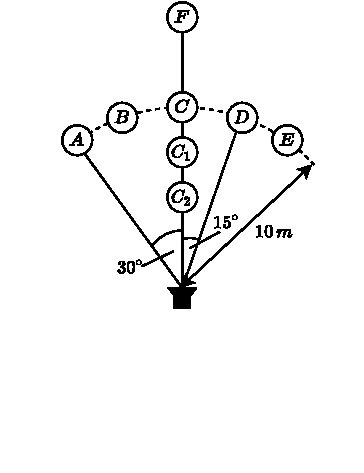
\includegraphics[trim=0mm 22mm 0mm 0mm]{images/6_Measurements/MeasurementSetup.pdf}
    \caption{Measurement setup final tests}
    \label{6_fig:measurement_setup_final}
\end{figure}
\subsection{Audio Quality}
To evaluate the audio quality as good as possible a grading system based on the swiss grading system was developed. This is shown in \ref{6.1.2_tab:audio_quality}.

\begin{center}
\begin{table}
\centering
\begin{tabular}{ |m{2.2cm}|m{2.2cm}|m{2.2cm}|m{2.2cm}|m{2.2cm}|m{2.2cm}|}
  \hline 
  1 & 2 & 3 & 4 & 5 & 6\\ 
  \hline
 Completely unrecognizable audio, very distorted and noisy & Hardly anything can be recognized, noise and distortion are dominant & Mostly recognizable audio, distortion and noise clearly hearable &  Acceptable hearing experience, speech recognizable without effort & Enjoyable hearing experience, appropriate for daily use &  Outstanding Hi-Fi audio quality, no noise hearable \\
 \hline
\end{tabular}
\caption{Audio quality grading system}
\label{6.1.2_tab:audio_quality}
\end{table}
\end{center}

\subsubsection{Measurements}
\begin{enumerate}
    \item General audio quality \\
    To test the general audio quality music and speech was played for the test person. The settings where set to default.
    \begin{center}
     \begin{table}[h!]
    \centering
    \begin{tabular}{ |c|c|c|}
      \hline 
      Test & Average & Variance \\ 
      \hline
     Music quality & 4.2 & 0.46 \\
     \hline
     Speech quality & 4.5 & 0.38 \\
     \hline
    \end{tabular}
    \caption{Audio quality score}
    \label{6.1.2_tab:music_audio_quality}
    \end{table}   
    \end{center}
    \item Equalizer \\
    For the second test the equalizer where changed and the music quality off each one was tested. The equalizer "Main" was not specifically tested but it is the default equalizer and is mentioned in \ref{6.1.2_tab:music_audio_quality_eq} as a comparison.
     \begin{center}
     \begin{table}[h!]
    \centering
    \begin{tabular}{ |c|c|c|}
      \hline 
      Test & Average & Variance \\ 
      \hline
     No equalizer & 4.1 & 0.67 \\
     \hline
     Equalizer: "Lowcut 300Hz" & 4.25 & 0.60 \\
     \hline
     Equalizer: "Sharp" & 4 & 0.66 \\
     \hline
     Equalizer: "Main" & 4.2 & 0.46 \\
     \hline
    \end{tabular}
    \caption{Audio quality of different equalizer}
    \label{6.1.2_tab:music_audio_quality_eq}
    \end{table}   
    \end{center}
    \item Modulation type \\
    In the last audio quality tests the two modulations types AM and MAM where compared. The other settings where again set to default
    \begin{center}
     \begin{table}[h!]
    \centering
    \begin{tabular}{ |c|c|c|}
      \hline 
      Test & Average & Variance \\ 
      \hline
     AM & 3.9 & 0.40 \\
     \hline
     MAM & 4.4 & 0.34 \\
     \hline
    \end{tabular}
    \caption{Audio quality of modulation types}
    \label{6.1.2_tab:music_audio_quality_mod}
    \end{table}   
    \end{center}
\end{enumerate}
A more detailed overview of the quality measurements can be seen in Figure \ref{6_fig:box_plot_quality}.
\begin{figure}
    \centering
    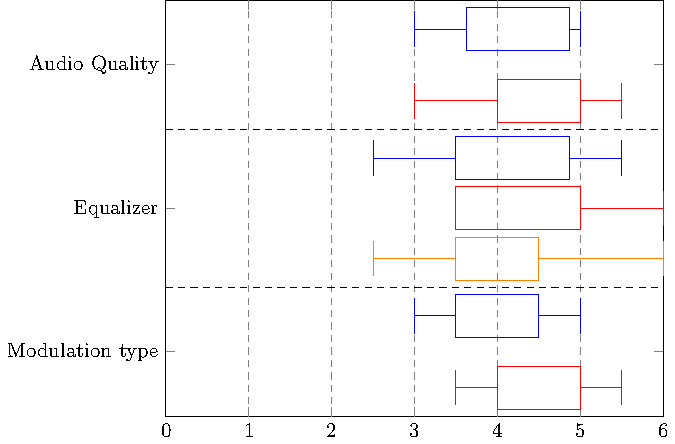
\includegraphics[width=0.7\textwidth]{images/6_Measurements/BoxPlotQuality.pdf}
    \caption{Box plot quality}
    \label{6_fig:box_plot_quality}
\end{figure}
\subsubsection{Evaluation}
The general audio quality test turned out well, as both music and speech where rated on average better than a acceptable hearing experience. Especially the audio quality of speech surprised us and showed us that this could be an important use case. In the equalizer test all results turned out to be about the same and statistically seen no huge difference between them. We think with more time and more testing better and more impressive equalizer settings can be found and this results can be improved. The modulation type test painted a strong picture that MAM modulation is the way to go. 
Overall, we are very pleased with these results and think a real alternative to conventional loudspeakers can be created with further improvements. 
\subsection{Audio Volume}
To evaluate the beam steering and directiviy as good as possible a grading system was developed. This is shown in \ref{6.1.3_tab:audio_volume}.

\begin{center}
\begin{table}
\centering
\begin{tabular}{ |m{2.2cm}|m{2.2cm}|m{2.2cm}|m{2.2cm}|m{2.2cm}|}
  \hline 
  -4 & -3 & -2 & -1 & 0\\ 
  \hline
Nearly nothing hearable, not noticeable volume level &	Noticeable if background is quiet (no one is talking) &	Strongly noticeable volume level, even with background noise (speech) &	Clearly hearable volume level & Very present volume level, strongly dominates background noise
\\
 \hline
\end{tabular}
\caption{Audio volume grading system}
\label{6.1.3_tab:audio_volume}
\end{table}
\end{center}
\subsubsection{Measurements}
Due to the absolute value of the volume being very objectiv the results of each individual test was normalized to be between 1, very loud, and zero, nothing audible. This means that the following list of test results says nothing about the absolute value of the loudspeaker.
\begin{enumerate}
    \item Directivity \\
    To test the directivity the test person had to rate the volume at every point (A, B, C, D and E). Once with no window applied and once with the Dolph-Chebyshev window, which should, in theory, generate a more directive beam.
    \begin{center}
     \begin{table}[h!]
    \centering
    \begin{tabular}{ |c|c|c|c|c|c|c}
      \hline 
      Test & A & B & C & D & E \\ 
      \hline
     No window & 0.34 & 0.57 & 1 & 0.66 & 0.43 \\
     \hline
     Dolph-Chebyshev & 0.32 & 0.5 & 1 & 0.54 & 0.34 \\
     \hline
    \end{tabular}
    \caption{Audio directivity}
    \label{6.1.2_tab:music_audio_volume_directivity}
    \end{table}   
    \end{center}
    \item Beam steering \\
    To test the beam steering two different tests where carried out.
    \subitem Point C\\
    In the first test the test person stood on Point C and the beam was steered to an angle of 0, 15 or 30 degrees. This was testes with no and the dolph chebyshev window.
    \begin{center}
     \begin{table}[h!]
    \centering
    \begin{tabular}{ |c|c|c|c|}
      \hline 
      Test & $0^\circ$ & $15^\circ$ & $30^\circ$ \\ 
      \hline
     No window & 0.98 & 0.8 & 0.83 \\
     \hline
     Dolph-Chebyshev & 1 & 0.72 & 0.70 \\
     \hline
    \end{tabular}
    \caption{Beamsteering Point C}
    \label{6.1.3_tab:music_audio_volume_steering_c}
    \end{table}   
    \end{center}
     \subitem Point A\\
    For the second test the test person stood on Point A and the beam was steered to an angle of 0, 15 or 30 degrees. This was testes with no and the dolph chebyshev window.
    \begin{center}
     \begin{table}[h!]
    \centering
    \begin{tabular}{ |c|c|c|c|}
      \hline 
      Test & $0^\circ$ & $15^\circ$ & $30^\circ$ \\ 
      \hline
     No window & 0.55 & 0.71 & 0.96 \\
     \hline
     Dolph-Chebyshev & 0.38 & 0.51 & 1 \\
     \hline
    \end{tabular}
    \caption{Beamsteering Point A}
    \label{6.1.3_tab:music_audio_volume_steering_A}
    \end{table}   
    \end{center}
\end{enumerate}
\subsubsection{Evaluation}
The directivity test showed that already at around $\pm 30^\circ$ the sound is almost only noticeable if the background is quiet. One can also see that the Dolph-Chebyshev window is, as expected, more directive. From the beam steering tests one saw that especially with no window it is very difficult to keep the point directly in front of the speaker quiet. This is in our opinion mainly due to the inherit directiviy of the loudspeaker. The second test, at point A, shows that the beam steering works as expected.   
\section{Ultrasonic Measurements}\label{6_sec:ultrasonic}
As an addition to the human expertise test a measurement series was carried out. Because we had no sound chamber on our disposal we had to carried out these measurements outside. But due to the surrounding noise a measurement in the hearable spectrum was impossible so all the measurements where carried out only with the carrier. Due to this and the difficulties of sound measurement without a ideal setup, measurement device and location these measurements have to be viewed with a grain of salt.
\subsection{Directivity}
The directivity of the ultrasound was measured with and without a window at 9 distinct points between $-30^\circ$ and $30^\circ$. The results of these measurements are shown in \ref{6.2.1_fig:Directivity_measurements}.
\begin{center}
    \begin{figure}[h!]
        \centering
        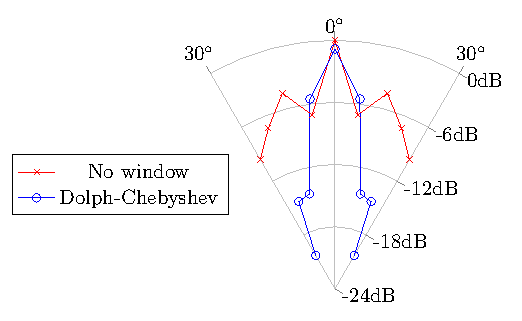
\includegraphics[width=0.5\textwidth]{images/6_Measurements/Polar_PlotDirectivity_Measurement.pdf}
        \caption{Directivity Measurements}
        \label{6.2.1_fig:Directivity_measurements}
    \end{figure}
\end{center}
\subsection{Beamsteering}
To measure the effects of the beamsteering the beam was once directed to $15^\circ$, as seen in Figure \ref{6.2.2_subfig:beamsteering_15}, and once directed to $30^\circ$, as seen in Figure \ref{6.2.2_subfig:beamsteering_30}. The dashed lines in both figures show the on the steered angle mirrored points to give a better feeling of how the beam looks like. Due to the inherit directional nature of the loudspeaker these dashed lines would in practice fall off a lot quicker than shown here. 
\begin{figure}[h!]
    \begin{minipage}{0.49\textwidth}
        \centering
        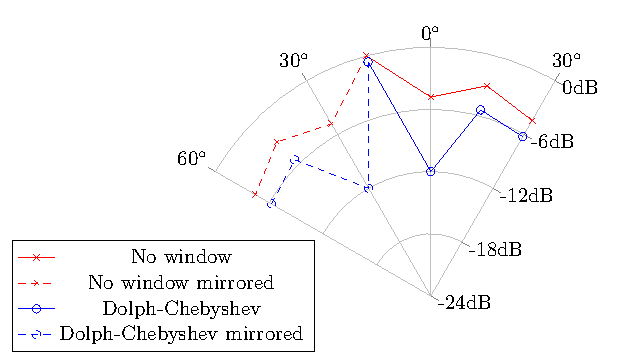
\includegraphics[width=\linewidth]{images/6_Measurements/Polar_PlotSteering_Measurement_15.pdf}
        \caption{Beam steered to 15$^\circ$}
        \label{6.2.2_subfig:beamsteering_15}
    \end{minipage}
    \begin{minipage}{0.49\textwidth}
        \centering
        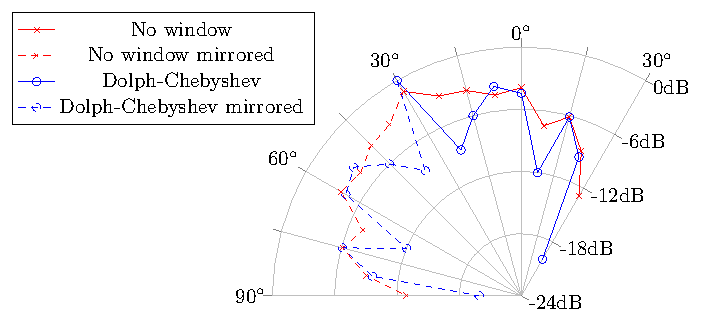
\includegraphics[width=\linewidth]{images/6_Measurements/Polar_PlotSteering_Measurement_30.pdf}
        \caption{Beam steered to 30$^\circ$}
         \label{6.2.2_subfig:beamsteering_30}
    \end{minipage}
\end{figure}
\subsection{Beamfocusing}
The beamfocusing was tested on the Points C1 (7.5m), C2 (5m) and F (15m). The results of this are shown in Figure \ref{6_fig:beamforming_measurements}.
\begin{figure}
    \centering
    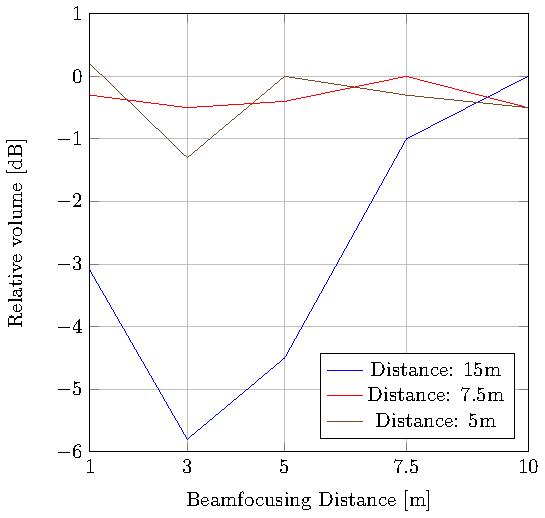
\includegraphics[width=0.5\textwidth]{images/6_Measurements/Beamfocusing.pdf}
    \caption{Beamfocusing measurements}
    \label{6_fig:beamforming_measurements}
\end{figure}
\subsection{Evaluation}
As already said due to the imperfect measurement setup these measurements have to be looked at critically. That said, the directivity and beam steering reflect the human expertise tests really well. In comparison to the calculations made in \ref{3_Parametric_array_Sec:Array_signal_processing} the measurements look similar, the main difference is the size of the grating lobe, which in our measurements is a lot smaller than calculated. This is most likely due to the directivity of the transducers not being the their assumed sinc function, as shown in Figure \ref{5_fig:directivity_transducer}. 
The beamfocusing on the other hand seems to only work if the distance to the loudspeaker is big enough but this theory has to be tested further in the future. 
\section{Transducer}
To get a better feeling for the transducers and to see how they behave under different circumstances a bunch of measurements where carried out. 
\subsection{Frequency Response}\label{6_sec:Frequency_response}
To be able to design more accurate equalizers the sound pressure level output at each frequency between 22.5 and 55 kHz was measured and is shown in \ref{6_Measurement_fig:Transducer_FR}. But again due to no access to a sound chamber these measurements have to be looked at critically.
\begin{figure}[h!]
    \centering
    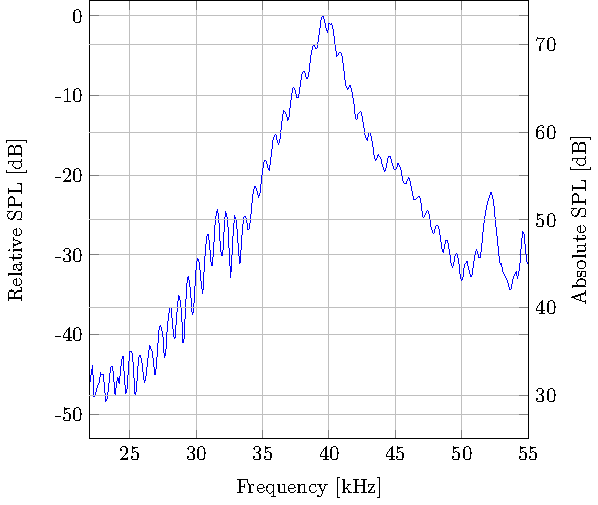
\includegraphics[width=0.5\textwidth]{images/6_Measurements/Transducer_Frequency_Respone.pdf}
    \caption{Frequency Response Transducer}
    \label{6_Measurement_fig:Transducer_FR}
\end{figure}
\subsection{Impedance Measurements}
To get information about the electrical side of the transducers a impedance measurement was carried out with a series of 20 transducers. It was measured using a vector network analyser. The results can be seen in Figure \todo{Figure Impedance Measurements}.
\subsection{Power Consumption}\label{6_subsec:Power_cons}
The power consumption of each of the 19 transducer lines is very important to access the output power of the loudspeaker. Over a $22 \, \Omega$ resistor in front of the transducer the current could be calculated. The voltage over the transducer and the voltage over the resistor was measured for 4 hours and it turned out that both these values where very constant. The voltage measured over the transducer was $U_T = 9.5 \,$V RMS and the voltage over the resistor $U_R = 1.78 \,$V RMS.
\newpage